\documentclass{article}
\usepackage{graphicx}
\usepackage{titletoc}
\usepackage{titlesec}
\usepackage{geometry} 
\usepackage{fontspec, xunicode, xltxtra}
\usepackage{float}
\usepackage{cite}
\usepackage{amsmath}
\usepackage{listings}
\usepackage{titletoc}
\usepackage{booktabs}

\geometry{left=3cm,right=3cm,top=3cm,bottom=3cm}
\DeclareMathOperator*{\argmin}{argmin}
\DeclareMathOperator*{\argmax}{argmax}
\DeclareMathOperator*{\logit}{logit}
\DeclareMathOperator*{\var}{var}
\DeclareMathOperator*{\cov}{cov}
\DeclareMathOperator*{\expec}{E}
\DeclareMathOperator*{\deriv}{d}
\DeclareMathOperator*{\const}{constant}

\begin{document}
\title{\textsf{Homework 8 for Bayesian Data Analysis}}
\author{Fan JIN\quad (2015011506)}
\maketitle

\section*{Question 11.3}
{
    \subsection*{Separate model and Pooled model:}
    {
        With the noninformative prior distribution, uniform for $(\theta, \log{\sigma})$,
        $$y_j | \theta, \sigma^2 \sim \mathrm{N}(\theta, \sigma^2),$$
        $$p(\theta, \sigma^2) \propto \sigma^{-2}.$$

        The conditional distributions are
        $$p(\theta | \sigma^2) \propto 1,$$
        $$p(\sigma^2 | \theta) \propto \sigma^{-2}.$$

        It follows that 
        $$p(\theta | \sigma^2, y) \propto 1 \cdot \mathrm{N}(\bar{y}, \sigma^2/n) \propto \exp{\left( -\frac{n}{2\sigma^2} (\bar{y}-\theta)^2 \right)},$$
        $$p(\sigma^2 | \theta, y) \propto \sigma^{-2-n} \cdot \exp{\left( -\frac{1}{2\sigma^2} \left[ (n-1)s^2 + n(\bar{y}-\theta)^2 \right] \right)}.$$

        \begin{itemize}

        \item For the separate model, plug in $y$ for the sixth machine only. 
        We can calculate the posterior distribution $\theta | y$ by simulation, using Metropolis-within-Gibbs on the two conditional distributions above. 
        \\ But we have no idea about the seventh machine, for each machine has its separate parameters. 
        Therefore, we cannot obtain the predictive distributions or the posterior mean for the seventh machine.

        \item For the pooled model, plug in $y$ for all the six machines. 
        We can calculate the posterior distribution $\theta | y$ by simulation, using Metropolis-within-Gibbs on the two conditional distributions above. 
        \\ And we use this posterior distribution to predict the seventh machine, for the machines have pooled parameters. 

        \end{itemize}
    }

    \subsection*{Hierarchical model:}
    {
        The four conditional distributions are given on p.289 of textbook:

        \begin{itemize}

        \item $$\theta_j | \mu, \sigma, \tau, y \sim \mathrm{N}(\hat{\theta}_j, V_{\theta_j}),$$ where
        $$\hat{\theta}_j = \frac{ \frac{1}{\tau^2}\mu + \frac{n_j}{\sigma^2}\bar{y}_{.j} }{ \frac{1}{\tau^2} + \frac{n_j}{\sigma^2} },$$
        $$V_{\theta_j} = \frac{1}{ \frac{1}{\tau^2} + \frac{n_j}{\sigma^2} }.$$

        \item $$\mu | \theta, \sigma, \tau, y \sim \mathrm{N}(\hat{\mu}, \tau^2/J),$$ where
        $$\hat{\mu} = \frac{1}{J} \sum_{j=1}^{J} \theta_j.$$

        \item $$\sigma^2 | \theta, \mu, \tau, y \sim \mathrm{Inv-}\chi^2 (n, \hat{\sigma}^2),$$ where
        $$n = \sum_{j=1}^{J} n_j,$$
        $$\hat{\sigma}^2 = \frac{1}{n} \sum_{j=1}^{J} \sum_{i=1}^{n_j} (y_{ij} - \theta_j)^2.$$

        \item $$\tau^2 | \theta, \mu, \sigma, y \sim \mathrm{Inv-}\chi^2 (J-1, \hat{\tau}^2),$$ where
        $$\hat{\tau}^2 = \frac{1}{J-1} \sum_{j=1}^{J} (\theta_j - \mu)^2.$$

        \end{itemize}

        Use Metropolis-within-Gibbs on the four conditional distributions above, we can draw $\theta_j$, $\mu$, $\sigma^2$, $\tau^2$ by simulation.
        The posterior distribution $\theta_j | y$ can be obtained immediately. 
        Then, we obtain $\mu | y$ and $\tau^2 | y$, which then give $\theta_7 | y$. 
        Finally, the posterior distribution $y_{i7} | y$ can be estimated, given $\sigma^2 | y$ obtained.
    }

    \subsection*{Reports}
    {
        Source code: ``src1.R''

        \begin{figure}[H]
            \centering
            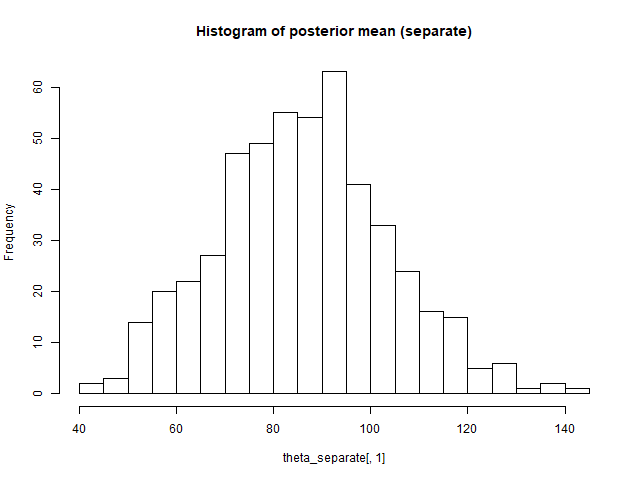
\includegraphics[width = 0.8\linewidth]{posterior_mean_separate.png}
            \caption{}
        \end{figure}
        \begin{figure}[H]
            \centering
            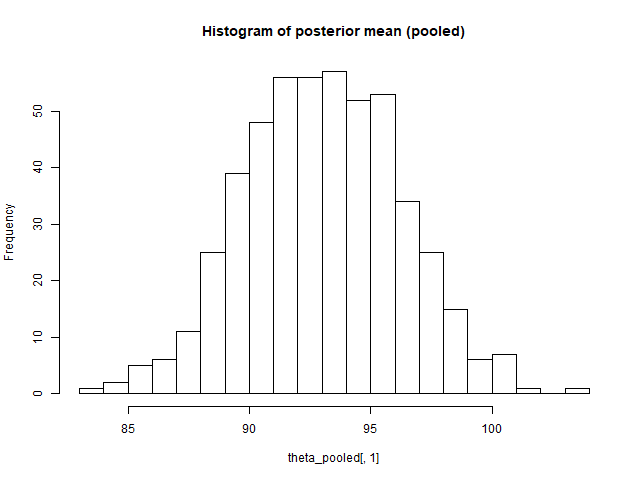
\includegraphics[width = 0.8\linewidth]{posterior_mean_pooled.png}
            \caption{}
        \end{figure}
        \begin{figure}[H]
            \centering
            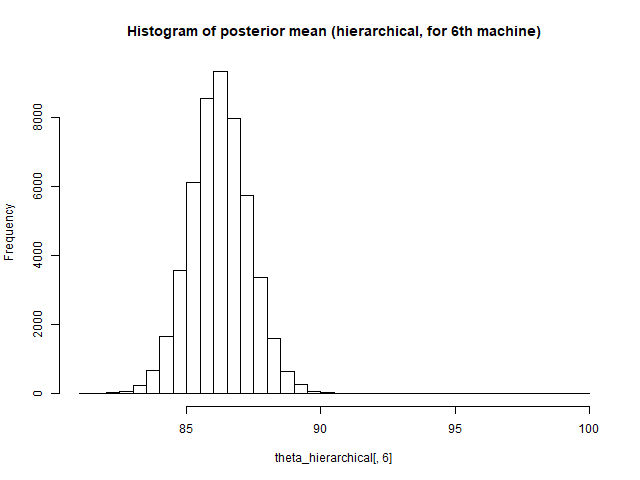
\includegraphics[width = 0.8\linewidth]{posterior_mean_hierarchical.png}
            \caption{}
        \end{figure}
        \begin{figure}[H]
            \centering
            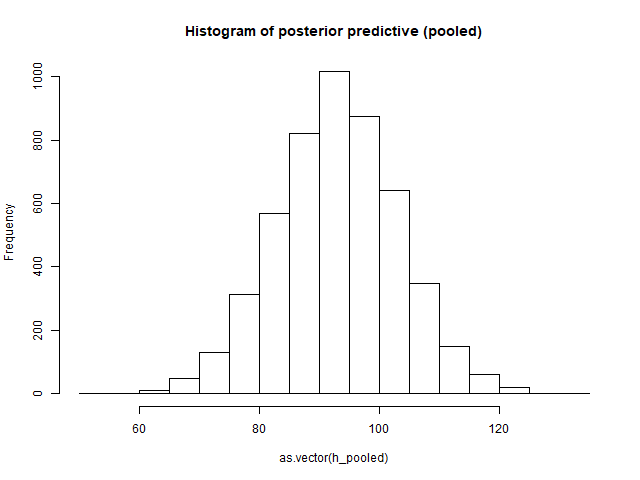
\includegraphics[width = 0.8\linewidth]{posterior_predictive_pooled.png}
            \caption{}
        \end{figure}
        \begin{figure}[H]
            \centering
            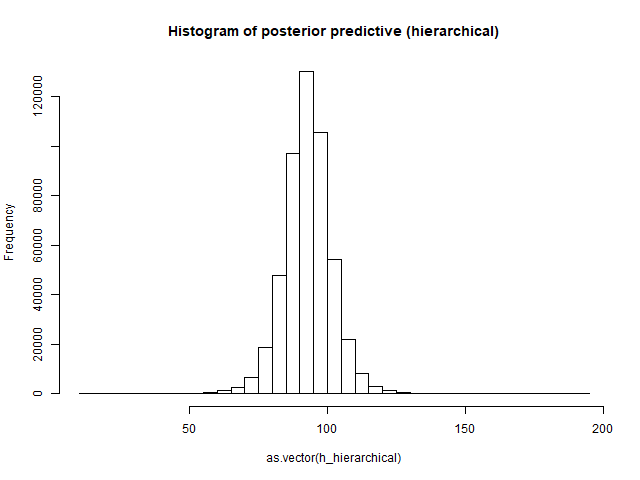
\includegraphics[width = 0.8\linewidth]{posterior_predictive_hierarchical.png}
            \caption{}
        \end{figure}
        \begin{figure}[H]
            \centering
            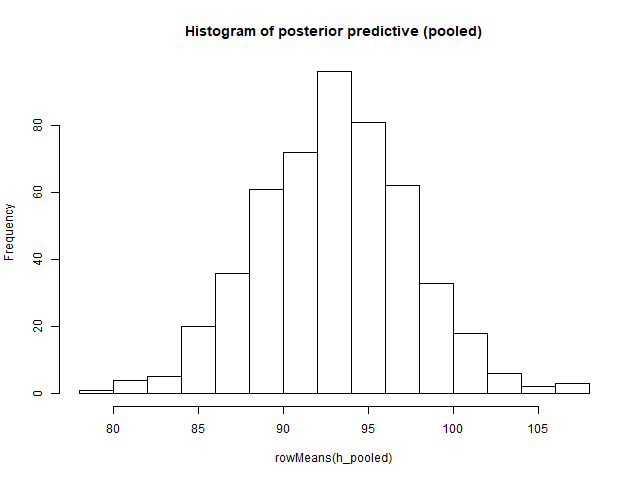
\includegraphics[width = 0.8\linewidth]{posterior_predictive_mean_pooled.png}
            \caption{}
        \end{figure}
        \begin{figure}[H]
            \centering
            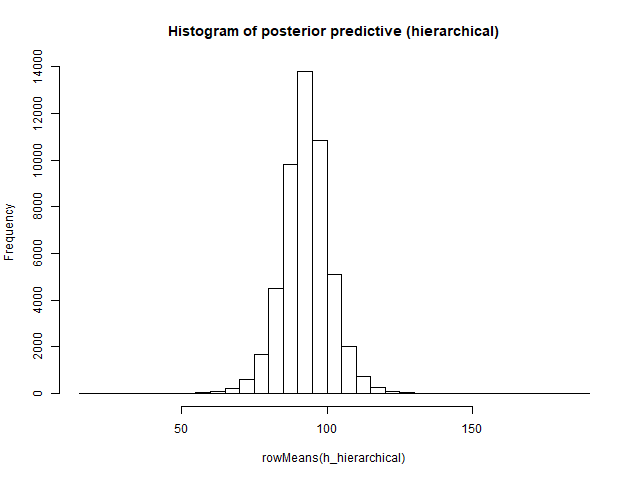
\includegraphics[width = 0.8\linewidth]{posterior_predictive_mean_hierarchical.png}
            \caption{}
        \end{figure}
    }
}

\section*{Random-walk Metroplis}
{
    Source code: ``src2.R''

    To make the adaptive tune of $\alpha$ and $\beta$ at each iteration, according to the empirical formula. For the first 20 iterations, we do not change the hyperparamters.

    \begin{lstlisting}[language=R]
    # Adapt
    if (i > 20) {
      tune$alpha = 2.4^2 * var(alpha_keep[1:i]) / 2
      tune$beta = 2.4^2 * var(beta_keep[1:i]) / 2
    }
    \end{lstlisting}

    The adaptived hyperparamters converge to $\alpha=0.04629154$ and $\beta=1.906087$.
    \begin{lstlisting}[language=R]
        $alpha
        [1] 0.04629154

        $beta
        [1] 1.906087
    \end{lstlisting}
}

\clearpage
\end{document}
